\documentclass[pdflatex, 11pt]{beamer}

\usepackage[utf8]{inputenc}
\usepackage[T1]{fontenc}
\usepackage[italian]{babel}
\usepackage{calligra}
\usepackage{graphicx}
\usepackage{tikz}
\usepackage{epstopdf}
\usepackage{spot}
\usepackage{multirow}
\usepackage{algorithm}% http://ctan.org/pkg/algorithms
\usepackage{algpseudocode}% http://ctan.org/pkg/algorithmicx

\graphicspath{{img/}}

\definecolor{links}{HTML}{2A1B81}
\hypersetup{colorlinks,linkcolor=links,urlcolor=links}

\mode<presentation>{
  \usetheme{Boadilla}
  \usecolortheme{beaver}
  \setbeamercovered{transparent=50}
  \setbeamertemplate{navigation symbols}{}
  \setbeamertemplate{itemize item}{\checkmark}
  \setbeamertemplate{itemize subitem}{-}
  \setbeamertemplate{enumerate items}[default]
}

\usebackgroundtemplate{
  \begin{tikzpicture}
    \node[opacity=0.05] {\includegraphics[scale=1]{img/logoUnifi.eps}};
  \end{tikzpicture}
}

\setspotlightstyle{rectangle}

\newcommand{\var}[1]{{\ttfamily#1}}% variable

\newenvironment<>{varblock}[2][\textwidth]{%
	\setlength{\textwidth}{#1}
	\begin{actionenv}#3%
		\def\insertblocktitle{#2}%
		\par%
		\usebeamertemplate{block begin}}
	{\par%
		\usebeamertemplate{block end}%
	\end{actionenv}}


\begin{document}

	\title[Motif Finding]{Analisi di algoritmi per il Motif Finding}
	\date[11 Dicembre 2015]{\flushright 11 Dicembre 2015}
	\institute[Università di Firenze]{
\includegraphics[width=5cm]{img/logoUnifiName.eps}}
	
	\author[Papini - Bani]{
		\begin{center}
			\begin{tabular}{lr}
				Tommaso \textsc{Papini}&Gabriele \textsc{Bani}\\
				\href{mailto:tommaso.papini1@stud.unifi.it}{tommaso.papini1@stud.unifi.it}&
				\href{mailto:gabriele.bani@stud.unifi.it}{gabriele.bani@stud.unifi.it}
			\end{tabular}
		\end{center}
	}
	
	\begin{frame}[plain]
		\titlepage
	\end{frame}
	
	\begin{frame}{Un po' di background}
		DNA:
		\begin{itemize}
			\item[$\bullet$] sequenza di \alert{\textbf{nucleotidi}}
			\item[$\bullet$] 4 tipi di nucleotide: A, T, C, G
			\item[$\bullet$] \alert{\textbf{\textit{l-mer}}}: sottosequenza di DNA di lunghezza $l$
		\end{itemize}
		\pause
		\begin{block}{Motifs}
			In biologia può essere necessario ricavare certe sequenze di DNA ``nascoste''
			\begin{itemize}
				\item pattern di nucleotidi ripetuti (l-mer)
				\item utili a capire determinati comportamenti biologici
				\begin{itemize}
					\item sequenze di attivazione di geni specifici
				\end{itemize}
			\end{itemize}
		\end{block}
	\end{frame}
	
	\begin{frame}{Il problema del Motif Finding}
		Il problema del \alert{\textbf{Motif Finding}} consiste nel ricavare un set di $t$ \alert{\textbf{l-mer}} da un insieme di $t$ sequenze di DNA.
		\pause
		\begin{block}{Input}
			\begin{itemize}
				\item[$\bullet$] $DNA$: matrice di nucleotidi $t \times n$
				\begin{itemize}
					\item $t$ sequenze di DNA
					\item ognuna di lunghezza $n$
				\end{itemize}
				\item[$\bullet$] $l$: lunghezza del motif cercato
			\end{itemize}
		\end{block}
		\pause
		\begin{block}{Output}
			\begin{itemize}
				\item $s=(s_1,s_2,\dots,s_t)$: lista di $t$ posizioni iniziali di l-mer il più simili tra loro
			\end{itemize}
		\end{block}
	\end{frame}
	
	\begin{frame}{Un primo esempio}
		\begin{center}
			\onslide<1>CGGGGCT\onslide<1,2>ATGCAACT\onslide<1>GGGTCGTCACATTCCCCTTTCGATA\\
			TTTGAGGGTGCCCAATAA\onslide<1,2>ATGCAACT\onslide<1>CCAAAGCGGACAAA\\
			GG\onslide<1,2>ATGCAACT\onslide<1>GATGCCGTTTGACGACCTAAATCAACGGCC\\
			AAGG\onslide<1,2>ATGCAACT\onslide<1>CCAGGAGCGCCTTTGCTGGTTCTACCTG\\
			AATTTTCTAAAAAGATTATAATGTCGGTCC\onslide<1,2>ATGCAACT\onslide<1>TC\\
			CTGCTGTACAACTGAGATCATGCTGC\onslide<1,2>ATGCAACT\onslide<1>TTCAAC\\
			TACATGATCTTTTG\onslide<1,2>ATGCAACT\onslide<1>TGGATGAGGGAATGATGC
		\end{center}
	\end{frame}
	
	\begin{frame}{Mutazioni random}
		\begin{center}						
			\onslide<.>CGGGGCT\onslide<1>ATcCAgCT\onslide<.>GGGTCGTCACATTCCCCTTTCGATA\\
			TTTGAGGGTGCCCAATAA\onslide<1>ggGCAACT\onslide<.>CCAAAGCGGACAAA\\
			GG\onslide<1>ATGgAtCT\onslide<.>GATGCCGTTTGACGACCTAAATCAACGGCC\\
			AAGG\onslide<1>AaGCAACc\onslide<.>CCAGGAGCGCCTTTGCTGGTTCTACCTG\\
			AATTTTCTAAAAAGATTATAATGTCGGTCC\onslide<1>tTGgAACT\onslide<.>TC\\
			CTGCTGTACAACTGAGATCATGCTGC\onslide<1>ATGCcAtT\onslide<.>TTCAAC\\
			TACATGATCTTTTG\onslide<1>ATGgcACT\onslide<.>TGGATGAGGGAATGATGC
		\end{center}
		\onslide<1>Come trovare l'l-mer più simile tra tutti?
	\end{frame}
	
	\begin{frame}{Allineamento}\tiny
		\begin{align*}					
			\onslide<.>CGGGGCT&\onslide<1>ATcCAgCT\onslide<.>GGGTCGTCACATTCCCCTTTCGATA\\
			\onslide<.>TTTGAGGGTGCCCAATAA&\onslide<1>ggGCAACT\onslide<.>CCAAAGCGGACAAA\\
			\onslide<.>GG&\onslide<1>ATGgAtCT\onslide<.>GATGCCGTTTGACGACCTAAATCAACGGCC\\
			\onslide<.>AAGG&\onslide<1>AaGCAACc\onslide<.>CCAGGAGCGCCTTTGCTGGTTCTACCTG\\
			\onslide<.>AATTTTCTAAAAAGATTATAATGTCGGTCC&\onslide<1>tTGgAACT\onslide<.>TC\\
			\onslide<.>CTGCTGTACAACTGAGATCATGCTGC&\onslide<1>ATGCcAtT\onslide<.>TTCAAC\\
			\onslide<.>TACATGATCTTTTG&\onslide<1>ATGgcACT\onslide<.>TGGATGAGGGAATGATGC
		\end{align*}
	\end{frame}
	
	\begin{frame}{Profilo e Consenso}
		\begin{center}
			\begin{tabular}{l l l l l l l l l l}
				\multirow{8}{*}{\textbf{Allineamento}} & & A & T & C & C & A & G & C & T\\
				& & G & G & G & C & A & A & C & T\\
				& & A & T & G & G & A & T & C & T\\
				& & A & A & G & C & A & A & C & C\\
				& & T & T & G & G & A & A & C & T\\
				& & A & T & G & C & C & A & T & T\\
				& & A & T & G & G & C & A & C & T\\
				\hline
				\multirow{4}{*}{\textbf{Profilo}} & \textbf{A} & 5 & 1 & 0 & 0 & 5 & 5 & 0 & 0\\
				& \textbf{T} & 1 & 5 & 0 & 0 & 0 & 1 & 1 & 6\\
				& \textbf{G} & 1 & 1 & 6 & 3 & 0 & 1 & 0 & 0\\
				& \textbf{C} & 0 & 0 & 1 & 4 & 2 & 0 & 6 & 1\\
				\hline
				\textbf{Consenso} & & A & T & G & C & A & A & C & T 
			\end{tabular}
		\end{center}
	\end{frame}
	
	\begin{frame}{Score}
		Come definire la ``bontà'' di un set di l-mer?
		\pause
		\begin{block}{Funzione score}
			Si definisce una funzione \alert{\textbf{score}} sul vettore $s=(s_1,s_2,\dots,s_t)$ di posizioni iniziali:
			\begin{equation*}
				Score(s,DNA)=\sum_{j=1}^{l}M_{P(s)}(j)
			\end{equation*}
			dove
			\begin{itemize}
				\item $P(s)$: matrice profilo su $s$
				\item $M_{P(s)}(j)$: elemento massimo nella colonna $j$-esima di $P(s)$
			\end{itemize}
		\end{block}
		\pause
		Si cerca il set di posizioni iniziali $s$ che \alert{\textbf{massimizzi}} $Score(s,DNA)$!
	\end{frame}
	
	\begin{frame}{Score: l'esempio di prima}
		\begin{center}
			\begin{tabular}{l l l l l l l l l l}
				\multirow{8}{*}{\textbf{Allineamento}} & & A & T & C & C & A & G & C & T\\
				& & G & G & G & C & A & A & C & T\\
				& & A & T & G & G & A & T & C & T\\
				& & A & A & G & C & A & A & C & C\\
				& & T & T & G & G & A & A & C & T\\
				& & A & T & G & C & C & A & T & T\\
				& & A & T & G & G & C & A & C & T\\
				\hline
				\multirow{4}{*}{\textbf{Profilo}} & \textbf{A} & 5 & 1 & 0 & 0 & 5 & 5 & 0 & 0\\
				& \textbf{T} & 1 & 5 & 0 & 0 & 0 & 1 & 1 & 6\\
				& \textbf{G} & 1 & 1 & 6 & 3 & 0 & 1 & 0 & 0\\
				& \textbf{C} & 0 & 0 & 1 & 4 & 2 & 0 & 6 & 1\\
				\hline
				\textbf{Consenso} & & A & T & G & C & A & A & C & T 
			\end{tabular}
		\end{center}
	\pause	$Score(s,DNA) = 5+5+6+4+5+5+6+6=42$
	\end{frame}
	
	\begin{frame}{Score}
		Quanto può valere lo \alert{\textbf{score}}?
		\pause
		\begin{equation*}
			Score(s,DNA) = \begin{cases}
				l\cdot t, & \mbox{nel caso migliore}\\
				\\
				\frac{l\cdot t}{4}, & \mbox{nel caso peggiore}
			\end{cases}
		\end{equation*}
		\begin{flushleft}
		\end{flushleft}
		\pause
		\begin{itemize}
			\item $lt$ corrisponde al caso in cui tutti gli l-mer sono identici
			\item $\frac{lt}{4}$ corrisponde al caso in cui gli l-mer siano diversi in tutte le posizioni
		\end{itemize}
	\end{frame}
	
	\begin{frame}{Algoritmi brute force}
		\begin{block}{Forza bruta}
			In informatica il metodo ``\alert{\textbf{forza bruta}}'' (o ricerca esaustiva della soluzione) è un algoritmo di risoluzione di un problema dato che consiste nel verificare tutte le soluzioni teoricamente possibili fino a che si trova quella effettivamente corretta.
		\end{block}
	\end{frame}
	
	\begin{frame}{Simple motif search}
		\begin{flushleft}
			\begin{block}{L'idea}
				Esamina tutte le possibili combinazioni delle posizioni di partenza $s$ e prendi quella con maggior \textit{Score}.
			\end{block}
		\end{flushleft}
		\pause
		\begin{flushleft}
			\begin{itemize}
				\item[$\bullet$] Posizioni iniziali: $s=(1,\dots,1)$
				\item[$\bullet$] Posizioni  finali: $s=((n-l+1),\dots,(n-l+1))$
			\end{itemize}
		\end{flushleft}
		\pause
		\begin{flushleft}
			Si utilizza il metodo $NextElement$ per passare da un elemento al successivo in ordine alfabetico.
		\end{flushleft}
	\end{frame}
	
	\begin{frame}{Simple motif search}{Pseudocodice}
		\begin{center}
			\begin{minipage}{7.7cm}
			    \begin{algorithmic}[1]
				    \Procedure{SimpleMotifSearch}{$DNA,t,n,l$}
					    \State $s\gets (1,1,\dots,1)$
					    \State $bestScore\gets Score(s,DNA)$
					    \While{$true$}
					    	\State $s\gets NextElement(s,t,n-l+1)$
					    	\If{$Score(s,DNA)>bestScore$}
					    		\State $bestScore\gets Score(s,DNA)$
					    		\State $bestMotif\gets s$
					    	\EndIf
					    	\If{$s=(1,1,\dots,1)$}
					    		\State \textbf{return} $bestMotif$
					    	\EndIf
					    \EndWhile
				    \EndProcedure
			    \end{algorithmic}
			\end{minipage}
	    \end{center}
	\end{frame}
	
	\begin{frame}{Simple motif search}{Complessità}
		Quante \alert{\textbf{iterazioni}} fa l'algoritmo?
		\pause
		\begin{flushleft}
			\begin{itemize}
				\item vengono esaminate tutte le possibili combinazioni
				\begin{itemize}
					\item $(n-l+1)$ possibili scelte per ogni posizione iniziale
					\item $t$ posizioni iniziali (una per ogni sequenza)
				\end{itemize}
				\pause
				\item $(n-l+1)^t$ possibili combinazioni di posizioni iniziali
			\end{itemize}
			\pause
		\end{flushleft}
		\begin{flushleft}
			Quanti \alert{\textbf{passi}} per calcolare \textit{Score}?
			\pause
			\begin{itemize}
				\item $tl$ per calcolare la matrice Profilo
				\pause
				\item $4l$ per calcolare \textit{Score}
			\end{itemize}
		\end{flushleft}
		\pause
		\begin{center}
			\begin{minipage}{3cm}
				\begin{block}{Costo}
					$$\mathcal{O}(tln^t)$$
				\end{block}
			\end{minipage}
		\end{center}
	\end{frame}
	
	\begin{frame}{Branch \& bound}
		\begin{block}{L'idea}
			Ottimizza \textit{Simple Motif Search} evitando di analizzare sequenze non ottimali
			\begin{itemize}
				\item enumerazione delle sequenze tramite \alert{\textbf{alberi}}
				\item funzione di \textit{Score ottimistico}
				\begin{itemize}
					\item \textit{Score parziale} su un nodo interno
					\item \textit{Score ideale} per le restanti posizioni
				\end{itemize}
			\end{itemize}
		\end{block}
	\end{frame}
	
	\begin{frame}{Branch \& bound}{Un esempio}
		\begin{center}
			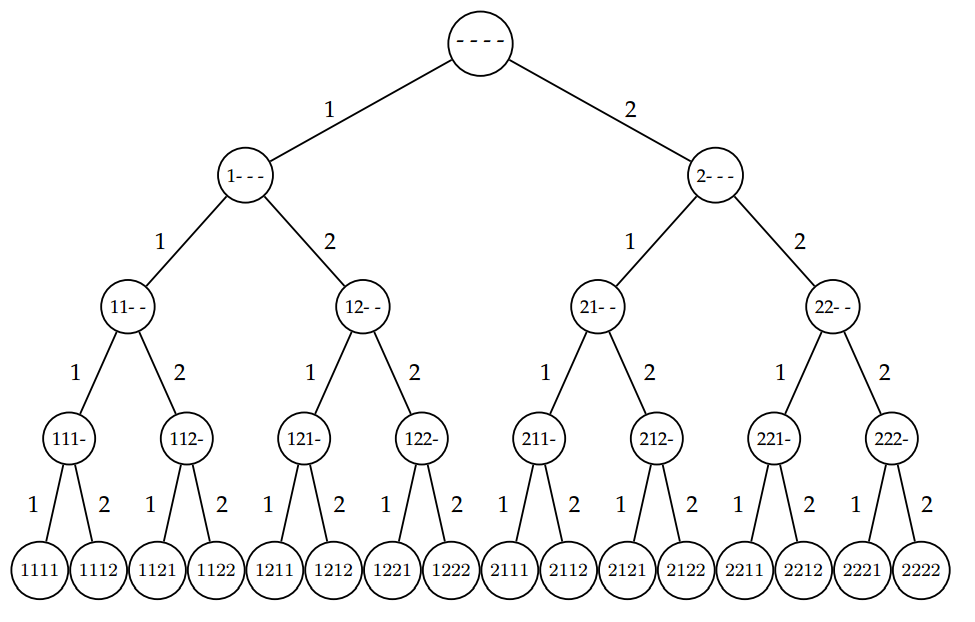
\includegraphics[scale=0.4]{albero.png}
		\end{center}
	\end{frame}
	
	\begin{frame}{Branch \& bound}{Un esempio}
		\begin{center}
			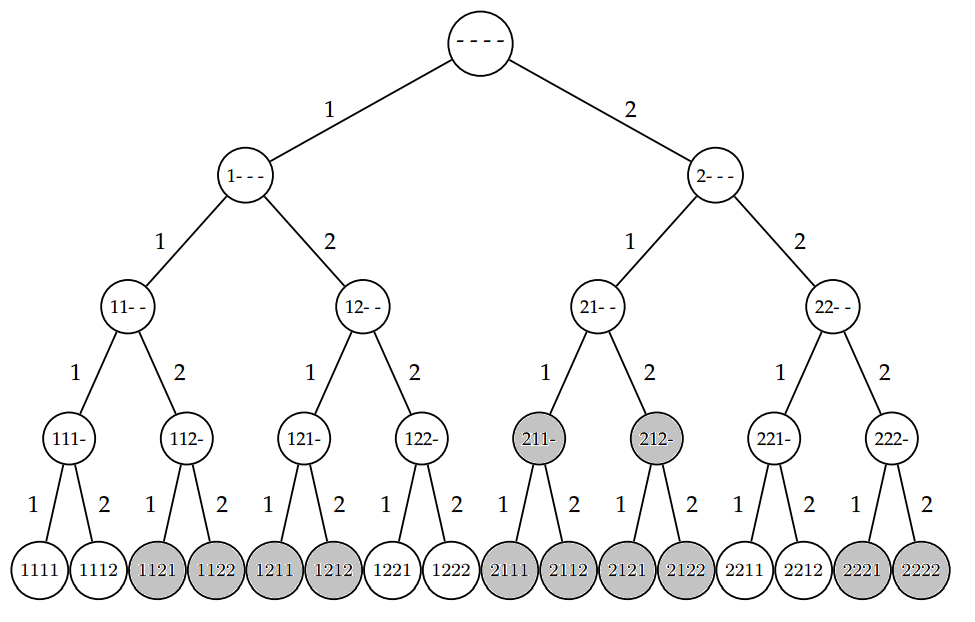
\includegraphics[scale=0.4]{albero2.png}
		\end{center}
	\end{frame}
	
	\begin{frame}{Branch \& bound}
		Si esegue una visita in profondità dell'albero
		\pause
		\begin{itemize}
			\item calcola lo \textit{Score ottimistico} per ogni nodo
			\pause
			\item scarta i sottoalberi con \textit{Score ottimistico} sub-ottimo
		\end{itemize}
		\pause
		\begin{block}{Score ottimistico}
			$$\mbox{Score ottimistico}=Score(s,i,DNA)+(t-i)\cdot l$$
			\begin{itemize}
				\item $Score(s,i,DNA)$: \textit{Score parziale} relativo alle prime $i$ sequenze di DNA
				\item $(t-i)\cdot l$: \textit{Score parziale} delle restanti posizioni (supponendole identiche)
			\end{itemize}
		\end{block}
		\pause
		\begin{itemize}
			\item $NextVertex$ per passare al prossimo vertice (DFS)
			\item $Skip$ per passare al prossimo vertice saltando il sottoalbero attuale
		\end{itemize}
	\end{frame}
	
	\begin{frame}{Branch \& bound}{Pseudocodice}
		\begin{center}\scriptsize
			\begin{minipage}{7.5cm}
			    \begin{algorithmic}[1]
				    \Procedure{BranchAndBoundMotifSearch}{$DNA,t,n,l$}
					    \State $s\gets (1,1,\dots,1)$
					    \State $bestScore\gets 0$
					    \State $i\gets 1$
					    \While{$i>0$}
							\If{$i<t$}
								\State $optimisticScore\gets Score(s,i,DNA)+(t-i)l$
								\If{$optimisticScore<bestScore$}
									\State $(s,i)\gets Skip(s,i,(n-l+1))$
								\Else
									\State $(s,i)\gets NextVertex(s,i,t,(n-l+1))$
								\EndIf
							\Else
								\If{$Score(s,DNA)>bestScore$}
									\State $bestScore\gets Score(s,DNA)$
									\State $bestMotif\gets s$
								\EndIf
								\State $(s,i)\gets NextVertex(s,i,t,(n-l+1))$
							\EndIf
					    \EndWhile
					    \State \textbf{return} $bestMotif$
				    \EndProcedure
			    \end{algorithmic}
			\end{minipage}
	    \end{center}
	\end{frame}
	
	\begin{frame}{Branch \& bound}{Complessità}
		Quante \alert{\textbf{iterazioni}}?
		\pause
		\begin{itemize}
			\item una per ogni nodo interno/foglia (caso pessimo)
			\pause
			\begin{itemize}
				\item $N=\frac{(n-l+1)^t-1}{(n-l+1)-1}$ nodi interni
				\item $L=(n-l+1)^t$ foglie
				\pause
			\end{itemize}
			\item $N+L$ passi totali
		\end{itemize}
		\pause
		Quanto \alert{\textbf{passi}} per calcolare \textit{Score}?
		\pause
		\begin{itemize}
			\item come prima!
		\end{itemize}
		\pause
		\begin{center}
			\begin{minipage}{3cm}
				\begin{varblock}{Costo}
					$$\mathcal{O}(tln^t)$$
				\end{varblock}
			\end{minipage}
		\end{center}
		\pause
		Come prima!
		\begin{itemize}
			\item più costoso nel caso pessimo
			\item conveniente se esegue tanti \textit{Skip}
		\end{itemize}
	\end{frame}
	
	\begin{frame}{Algoritmi greedy}
		\begin{block}{Greedy}
			Un algoritmo \alert{\textbf{greedy}} è un algoritmo che cerca di ottenere una soluzione ottima da un punto di vista globale attraverso la scelta della soluzione più golosa ad ogni passo locale
		\end{block}
	\end{frame}
	
	\begin{frame}{Greedy motif search}
		\begin{block}{L'idea}
			Scansiona ogni sequenza di DNA una sola volta e prendi l'l-mer che massimizza lo \textit{Score parziale}
		\end{block}
		\pause
		\begin{itemize}
			\item ciclo di inizializzazione per calcolare i primi due l-mer
			\begin{itemize}
				\item brute force
			\end{itemize}
			\pause
			\item i restanti l-mer scelti secondo lo \textit{Score parziale}
		\end{itemize}
	\end{frame}
	
	\begin{frame}{Greedy motif search}{Pseudocodice}
		\begin{center}\scriptsize
			\begin{minipage}{8.6cm}
			    \begin{algorithmic}[1]
				    \Procedure{GreedyMotifSearch}{$DNA,t,n,l$}
				    	\State $bestMotif\gets (1,1,\dots,1)$
					    \State $s\gets (1,1,\dots,1)$
					    \For{$s[1]\gets 1$ \textbf{to} $n-l+1$}
					    	\For{$s[2]\gets 1$ \textbf{to} $n-l+1$}
					    		\If{$Score(S,2,DNA)>Score(bestMotif,2,DNA)$}
					    			\State $bestMotif[1]\gets s[1]$
					    			\State $bestMotif[2]\gets s[2]$
					    		\EndIf
					    	\EndFor
					    \EndFor
					    \State $s\gets bestMotif$
					    \For{$i\gets 3$ \textbf{to} $t$}
					    	\For{$s[i]\gets 1$ \textbf{to} $n-l+1$}
					    		\If{$Score(S,i,DNA)>Score(bestMotif,i,DNA)$}
					    			\State $bestMotif[i]\gets s[i]$
					    		\EndIf
					    	\EndFor
					    	\State $s[i]\gets bestMotif[i]$
					    \EndFor
					    \State \textbf{return} $bestMotif$
				    \EndProcedure
			    \end{algorithmic}
			\end{minipage}
	    \end{center}
	\end{frame}
	
	\begin{frame}{Greedy motif search}{Complessità}
		Quanti \alert{\textbf{passi}} fanno i primi due cicli?
		\pause
		\begin{itemize}
			\item $(n-l+1)$ cicli ognuno
			\pause
			\item in ogni ciclo si invoca \textit{Score} due volte
			\begin{itemize}
				\item $2(tl+4l)$ passi
			\end{itemize}
			\pause
		\end{itemize}
		Quanti \alert{\textbf{passi}} fanno i secondi due cicli?
		\pause
		\begin{itemize}
			\item $(t-3)$ passi il ciclo esterno
			\pause
			\item $(n-l+1)$ passi il ciclo interno
			\pause
			\item in ogni ciclo si invoca \textit{Score} due volte
			\begin{itemize}
				\item come prima!
			\end{itemize}
			\pause
		\end{itemize}
		\begin{center}
			\begin{minipage}{4cm}		
				\begin{varblock}{Costo}
					\begin{align*}
						&\mathcal{O}(tln^2 + t^2ln) \uncover<2->{=}\\
						\pause
						\uncover<2->{=\;} & \uncover<2->{\mathcal{O}(tln(n+t))}\\
					\end{align*}
				\end{varblock}
			\end{minipage}
		\end{center}
	\end{frame}
	
	\begin{frame}{Greedy motif search}{Esattezza e approssimazione}
		\textit{GreedyMotifSearch} potrebbe non calcolare la soluzione ottima!
		\begin{itemize}
			\item algoritmo greedy approssimato (non esatto)
		\end{itemize}
		\pause
		Di quanto viene approssimata la soluzione trovata?
		\begin{itemize}
			\item fattore di approssimazione sconosciuto!
		\end{itemize}
		\pause
		\begin{block}{CONSENSUS}
			Esiste un'implementazione (CONSENSUS) di \textit{GreedyMotifSearch}
			\begin{itemize}
				\item risultati spesso vicini all'ottimo
				\item complessità molto bassa
			\end{itemize}
		\end{block}
	\end{frame}
	
	\begin{frame}{Algoritmi randomizzati}
		\begin{block}{Random}
			Gli algoritmi \alert{\textbf{randomizzati}} sono algoritmi che impiegano un certo grado di casualità durante la loro esecuzione al fine di ottenere delle buone prestazioni nel caso medio
		\end{block}
	\end{frame}
	
	\begin{frame}{Greedy profile motif search}
		\begin{block}{L'idea}
			Crea un profilo su un vettore $s$ casuale, calcola, per ogni sequenza, l'l-mer che ha più probabilità di aver generato tale profilo e ripeti sul nuovo profilo ottenuto
		\end{block}
		\pause
		Come si definisce la  probabilità che un l-mer $a$ abbia generato un profilo $P$?
		\pause
		\begin{itemize}
			\item $Prob(a|P)=\prod_{i=1}^{l}p_{a_i,i}$
			\item con $P(s)=(p_{ij})$ matrice profilo costruita su $s$ 
		\end{itemize}
	\end{frame}
	
	\begin{frame}{Greedy profile motif search}{Pseudocodice}
		\begin{center}
			\begin{minipage}{10.5cm}
			    \begin{algorithmic}[1]
				    \Procedure{GreedyProfileMotifSearch}{$DNA,t,n,l$}
				    	\State $s\gets$  vettore casuale di posizioni iniziali in $DNA$
				    	\State $P\gets P(s)$
				    	\State $bestScore\gets 0$
				    	\While{$Score(s,DNA)>bestScore$}
				    		\State $bestScore\gets Score(s,DNA)$
				    		\For{$i\gets 1$ \textbf{to} $t$}
				    			\State $a\gets $ l-mer dell'i-esima sequenza più probabile per $P$
				    			\State $s[i]\gets $ posizione iniziale di $a$
				    		\EndFor
				    	\EndWhile
				    	\State \textbf{return} $s$
				    \EndProcedure
			    \end{algorithmic}
			\end{minipage}
	    \end{center}
	\end{frame}
	
	\begin{frame}{Greedy profile motif search}{Complessità}
		Quante \alert{\textbf{iterazioni}} esegue il \textit{while}?
		\pause
		\begin{itemize}
			\item al più $t\cdot(n-l+1)$
			\pause
			\item in ogni ciclo si calcola \textit{Score} due volte
			\begin{itemize}
				\item $2(tl+4l)$ passi
			\end{itemize}
			\pause
			\item ciclo \textit{for}
			\pause
			\begin{itemize}
				\item $t$ passi totali
				\item in ogni passo  si cerca l'l-mer con probabilità  più alta
				\pause
				\begin{itemize}
					\item $(n-l+1)$ l-mer da controllare
					\item il calcolo di ogni probabilità richiede $l$ passi
				\end{itemize}
				\pause
			\end{itemize}
		\end{itemize}
		\begin{center}
			\begin{minipage}{3cm}
				\begin{varblock}{Costo}
					$$\mathcal{O}(ln^2t^2)$$
				\end{varblock}
			\end{minipage}
		\end{center}
	\end{frame}
	
	\begin{frame}{Gibbs sampling}
		\begin{block}{L'idea}
			Simile a \textit{GreedyProfileMotifSearch} ma aggiornando ad ogni passo una sola sequenza (scelta in modo casuale) anziché tutte e scegliendo l'l-mer migliore in modo  probabilistico e non greedy
		\end{block}
	\end{frame}
	
	\begin{frame}{Gibbs sampling}{Pseudocodice}
		\begin{center}
			\begin{minipage}{11.5cm}
			    \begin{algorithmic}[1]
				    \Procedure{GibbsSampling}{$DNA,t,n,l$}
				    	\State $s\gets$  vettore casuale di posizioni iniziali in $DNA$
				    	\Repeat
				    		\State $x\gets$ indice di una sequenza di DNA scelta casualmente
				    		\State $P\gets P(s)$ calcolata sulle restanti $t-1$ sequenze
				    		\For{$i\gets 1$ \textbf{to} $n-l+1$}
				    			\State $a\gets$ l-mer della sequenza $x$-esima con posizione iniziale $i$
				    			\State $p_i\gets $ probabilità che $a$ abbia generato $P$
				    		\EndFor
				    		\State $j\gets$ scelta casuale sulla distribuzione $(p_1,p_2,\dots,p_{n-l+1})$
				    		\State $s[x]\gets j$
				    	\Until{convergenza}
				    	\State \textbf{return} $s$
				    \EndProcedure
			    \end{algorithmic}
			\end{minipage}
	    \end{center}
	\end{frame}
	
	\begin{frame}{Gibbs sampling}{Complessità}
		Assumendo la stessa funzione obiettivo di \textit{GreedyProfileMotifSearch}:
		\begin{itemize}
			\item stessi passi di prima
			\item eccetto il ciclo sulle sequenze
			\begin{itemize}
				\item viene analizzata una sola sequenza per ciclo
			\end{itemize}
		\end{itemize}
		\pause
		\begin{center}
			\begin{minipage}{3cm}
				\begin{varblock}{Costo}
					$$\mathcal{O}(ln^2t)$$
				\end{varblock}
			\end{minipage}
		\end{center}
	\end{frame}
	
	\begin{frame}{Conclusioni}
		\renewcommand{\arraystretch}{2.3}
		\definecolor{darkgreen}{HTML}{008000}
		\begin{center}
			\begin{tabular}{ll|c|c|}
				&  & Costo & Esattezza\\
				\hline
				\multirow{2}{*}{\textbf{Forza bruta}} & \textbf{Simple MS} & $\mathcal{O}(tln^t)$ & {\Large \color{darkgreen} \checkmark}\\
				\cline{2-4}
				& \textbf{Branch \& Bound} & $\mathcal{O}(tln^t)$ & {\Large \color{darkgreen} \checkmark}\\
				\hline
				\textbf{Greedy} & \textbf{Greedy MS} & $\mathcal{O}(tln(n+t))$ & \\
				\hline
				\multirow{2}{*}{\textbf{Randomizzati}} & \textbf{Greedy Profile MS} & $\mathcal{O}(ln^2t^2)$ & \\
				\cline{2-4}
				& \textbf{Gibbs Sampling} & $\mathcal{O}(ln^2t)$ & \\
				\hline
			\end{tabular}
		\end{center}
	\end{frame}
	
	\begin{frame}
		\begin{center}
			\textbf{\fontsize{50}{60}\selectfont Fine!}\\[1cm]
			\pause
			\begin{flushleft}
			\end{flushleft}
			\begin{flushleft}
			\end{flushleft}
			{\huge Domande?}
		\end{center}
	\end{frame}
	
	\begin{frame}{Appendice}{NextElement}
		\begin{center}
			\begin{minipage}{5.8cm}
				\begin{algorithmic}[1]
					\Procedure{NextElement}{$a, L, k$}
					\For{$i\gets L$ \textbf{to} $1$}
						\If{$a[i] < k$}
							\State $a[i] \gets a[i] + 1$
							\State \textbf{return} $a$
						\EndIf
						\State $a[i] \gets 1$
					\EndFor
					\State \textbf{return} $a$				
					\EndProcedure
				\end{algorithmic}
			\end{minipage}
		\end{center}	
	\end{frame}
	
	\begin{frame}{Appendice}{NextVertex}
		\begin{center}
			\begin{minipage}{5.8cm}
				\begin{algorithmic}[1]
					\Procedure{NextVertex}{$a, i, L, k$}
					\If{$i < L$}
						\State $a[i+1] \gets 1$
						\State \textbf{return} $(a, i+1)$
					\Else
						\For{$j \gets L$ \textbf{to} $1$}
							\If{$a[j] < k $}
								\State $a[j] \gets a[j] + 1$
								\State \textbf{return} $(a, j)$
							\EndIf
						\EndFor
					\EndIf
					\State \textbf{return} $(a, 0)$				
					\EndProcedure
				\end{algorithmic}
			\end{minipage}
		\end{center}	
	\end{frame}	

	\begin{frame}{Appendice}{Skip}
		\begin{center}
			\begin{minipage}{4.8cm}
				\begin{algorithmic}[1]
					\Procedure{Skip}{$a, i, k$}
						\For{$j \gets i$ \textbf{to} $1$}
							\If{$a[j] < k$}
								\State $a[j] \gets a[j] + 1$
								\State \textbf{return} $(a,j)$
							\EndIf
						\EndFor										
						\State \textbf{return} $(a, 0)$				
					\EndProcedure
				\end{algorithmic}
			\end{minipage}
		\end{center}	
	\end{frame}	


\end{document}